\documentclass[conference]{IEEEtran}
\IEEEoverridecommandlockouts

\usepackage{cite}
\usepackage{amsmath,amssymb,amsfonts}
\usepackage{algorithm}
\usepackage{algpseudocode}
\usepackage{graphicx}
\usepackage{booktabs}
\usepackage{multirow}
\usepackage{xcolor}
\usepackage{url}
\usepackage{tikz}
\usetikzlibrary{arrows.meta,positioning,fit,calc,shapes.geometric}
\usepackage{pgfplots}
\pgfplotsset{compat=1.17}
\usepgfplotslibrary{groupplots}

\newcommand{\That}{\hat{T}}
\newcommand{\dbar}{\bar{d}}
\newcommand{\shat}{\hat{s}}
\newcommand{\ahat}{\hat{a}}
\newcommand{\Acal}{\mathcal{A}}
\newcommand{\Ccal}{\mathcal{C}}
\newcommand{\rhomin}{\rho_{\min}}
\newcommand{\stlG}{\mathbf{G}}
\newcommand{\stlU}{\mathbf{U}}

\begin{document}

\title{Predictive Verification in a Shielded SDN Control Loop:\\
A Stage-1 Prototype of a Verifiable Generative Control Plane}

\author{\IEEEauthorblockN{Venkatesh V (23BEC060),
Kalyan J (23BEC022),
Dileep A (23BEC003),\\
Lakshmi Prasad D (23BEC018)\IEEEauthorrefmark{1},
S Siva Tejananda Reddy (23BEC053)}
\IEEEauthorblockA{\textit{Department of Electronics and Communication Engineering}\\
\textit{Indian Institute of Information Technology Dharwad}\\
Dharwad, Karnataka, India\\
\IEEEauthorrefmark{1}Contact author: 23bec018@iiitdwd.ac.in}
}

\maketitle

\begin{abstract}
A controller that proposes SDN actions, whether learned, generative or hand-written,
can produce a configuration that is valid now but breaks a capacity limit or a
latency requirement a few slots later. We study whether \emph{predictive
verification} can keep such actions off the network: every candidate is rolled ten
slots ahead with a nominal queueing model and a fallback policy, checked against
hard constraints and Signal Temporal Logic (STL) latency intents, and certified only
if every intent keeps a robustness margin; a single enforcing applier installs only
certified actions, or the fallback. We built a Stage-1 prototype of the verifiable
generative control plane in which the learned generator and world model of the
original formulation are replaced by heuristic candidates and an analytic model, so
that the verification path can be tested in isolation. On a six-switch, three-slice
topology we compare five controllers that receive identical candidates, in a
simulator (six scenarios, five seeds, five held-out seeds, two ablations) and on
Mininet with Open vSwitch. Under a background surge, routing the same candidates
through the shield reduced violation slots from 16.4 to 0.8 per 60-slot run in
simulation and from 4.2 to 0.6 on the emulated network, at 22--33\,ms of
verification per one-second slot. The shield did not outperform a capacity-aware
heuristic, which achieved the same outcomes, and with a fixed fallback that did not
fit the surge it gave no protection at all. When the network differed structurally
from the model, it certified unsafe actions in every slot, and recalibrating the
model did not fix this. The prototype therefore shows that the certified path
removes the dependence of safety on the generator, but not on the model or the
fallback.
\end{abstract}

\begin{IEEEkeywords}
software-defined networking, network slicing, signal temporal logic, runtime
verification, safety shield, model predictive control, Mininet
\end{IEEEkeywords}

% =====================================================================
\section{Introduction}

In software-defined networking (SDN), routing and rate-limiting decisions are taken
by a logically central controller and installed on switches through an open
interface \cite{mckeown2008openflow,kreutz2015sdn}. Sliced 5G and planned 6G
networks push this further: each slice has its own latency and throughput
requirements, and demand and background traffic change from one control interval to
the next \cite{foukas2017slicing,saad2020vision6g}. Learned controllers and, more
recently, generative models are being proposed to choose these configurations
\cite{boutaba2018mlnet,mao2016deeprm,leivadeas2023ibn,mondal2023llmconfig}.

A proposed action can be a valid configuration and still be a bad decision. Give
the broadband slice a 150\,Mbit/s reservation on a 200\,Mbit/s path. The rules are
well formed and, when installed, the path may be lightly used. If unmanaged traffic
then arrives on the same path, the link overloads within a slot and the slice's
queueing delay rises far above its bound. Data-plane verifiers
\cite{kazemian2012hsa,khurshid2013veriflow} establish that rules are reachable,
loop-free and isolated; they do not predict how load and latency will evolve once
the rules are in place. A controller that may hallucinate, as generative models do,
needs a check of the second kind.

The problem formulation of our course project \cite{vgcp_formulation} proposes a
\emph{verifiable generative control plane} in which a generative policy proposes
candidates and a verification shield accepts a candidate only if, rolled forward
with a conservative nominal model and continued by a fallback policy, it satisfies
hard constraints and STL intents with a robustness margin. If no candidate is
certified, the fallback is applied. The formulation guarantees safety only under
three assumptions: the horizon covers every intent, the shield is sound, and the
fallback is always feasible.

This paper asks what such a shield achieves in practice, before any learning is
involved:

\begin{quote}
\emph{Can predictive verification of candidate actions keep actions that violate
configured constraints or temporal service requirements off the certified control
path, and under which conditions does that protection fail?}
\end{quote}

\noindent We make the question testable with three hypotheses, each answered by a
specific comparison in Section~\ref{sec:results}:

\begin{itemize}
\item[\textbf{H1}] \emph{Prevention.} When the nominal model is adequate, routing
a generator's candidates through the shield prevents the outcome violations that
the same candidates cause when applied without verification. Test: shielded versus
unshielded controllers on identical candidates (s2, s6).
\item[\textbf{H2}] \emph{Model dependence.} Certification is only as reliable as the
nominal model: when the network differs structurally from the model, certified
actions can violate the intents, and rescaling the model does not repair this.
Test: scenario s5 and the calibration study.
\item[\textbf{H3}] \emph{Fallback dependence.} The shield helps only if the
fallback used in its rollouts is itself feasible. Test: an ablation that changes only
the fallback (static versus capacity-aware) with the generator, model and
verification logic unchanged (s2, s6).
\end{itemize}

\noindent Two further questions, the verification cost and how often the shield is
unnecessarily conservative, are measured alongside.

We deliberately did not start with a learned generator. With a learned generator
and a learned model, a failure could come from either of them or from the shield.
Our prototype uses heuristic candidates, including a deliberately greedy one and
random actions that play the role of hallucinated proposals, and an analytic
queueing model whose errors can be traced. The contributions are:

\begin{itemize}
\item an implementation of the formulation's local feasibility certificate as a
shield that issues machine-readable certificates, and a single enforcing applier
that is the only shielded path to the network (Section~\ref{sec:method});
\item the interpretations needed to make the formulation executable, stated
explicitly (Section~\ref{sec:formulation});
\item an evaluation of H1--H3 on a simulator and on Mininet/Open vSwitch against four
baselines that receive identical candidates, including a strong hand-written
heuristic, with held-out seeds and ablations of the fallback, the selection rule and
model calibration (Sections~\ref{sec:setup}--\ref{sec:analysis});
\item negative findings reported as such: the shield matched but did not beat the
heuristic, it gave no protection with an infeasible fallback, it certified unsafe
actions under a wrong model, and part of the emulated evidence remains open.
\end{itemize}

The prototype, configurations, experiment reports and tests are public
\cite{vgcp_repo}.

% =====================================================================
\section{Related Work}

\emph{SDN control and data-plane verification.} OpenFlow
\cite{mckeown2008openflow} and SDN controllers \cite{kreutz2015sdn,berde2014onos}
make it possible to change paths and rate limits programmatically. Header space
analysis \cite{kazemian2012hsa} and VeriFlow \cite{khurshid2013veriflow} verify
data-plane invariants, statically or as rules change. These tools answer whether a
configuration is well formed. Our shield asks a different question, how load and
latency will evolve over a horizon once a configuration is installed, and its
routing-validity check is a much simpler version of what they verify.

\emph{Learning-based and intent-based network management.} Machine learning has
been applied to traffic classification, routing and resource management
\cite{boutaba2018mlnet}, for example with deep reinforcement learning for resource
allocation \cite{mao2016deeprm}. Intent-based networking translates operator goals
into configurations \cite{leivadeas2023ibn}, and recent work studies what language
models need to produce correct router configurations \cite{mondal2023llmconfig}.
O-RAN exposes similar closed loops in the radio access network
\cite{polese2023oran}. We do not propose a generator; we study the check that such a
generator's output would pass through.

\emph{Runtime verification and temporal logic.} Runtime verification checks an
execution against a specification as it unfolds \cite{leucker2009rv}. STL was
introduced for monitoring real-valued signals \cite{maler2004stl}, and its
quantitative robustness semantics gives a signed margin by which a signal satisfies
or violates a formula \cite{fainekos2009robustness,donze2010robust}. We use these
semantics unchanged on discrete control slots. Our use differs from monitoring in one
respect: we evaluate the formula on a \emph{predicted} trajectory before acting,
not on the observed one afterwards.

\emph{Predictive and safe control.} Constrained model predictive control (MPC)
optimizes inputs over a horizon subject to constraints, and establishes recursive
feasibility through a terminal set and controller \cite{mayne2000mpc}. STL
specifications can be encoded into MPC \cite{raman2014stlmpc}. Our rollout,
which applies the candidate once and a fallback afterwards, resembles the terminal
controller construction, but we evaluate a handful of proposed candidates instead of
optimizing, and we do not establish recursive feasibility; we measure how often it
fails. The Simplex architecture \cite{sha2001simplex} pairs a high-performance
controller with a verified safety controller and a switching rule, an idea close to
our certified path and fallback. Shielding for reinforcement learning
\cite{alshiekh2018shielding,garcia2015saferl} and control barrier functions
\cite{ames2017cbf} also override unsafe actions, given a model of the safe set or
the dynamics. All of these inherit the correctness of that model, which is the
dependence our H2 measures.

% =====================================================================
\section{Problem Scenario}
\label{sec:scenario}

We consider a transport network serving three slices: URLLC (ultra-reliable
low-latency), eMBB (enhanced mobile broadband) and mMTC (massive machine-type
communication). The topology (Fig.~\ref{fig:topology}) has six switches and three
paths from ingress $s_1$ to egress $s_5$: path A (two 50\,Mbit/s links, 0.1\,ms
propagation each), path B (two 200\,Mbit/s links, 5\,ms each) and path C (three
50\,Mbit/s links, 2\,ms each). By default URLLC uses A, eMBB uses B and mMTC uses C.
Nominal demand is 2, 80 and 2\,Mbit/s for URLLC, eMBB and mMTC, with 5\,\% noise.

Every second (one control slot), the controller chooses for each slice a path, a
rate budget enforced by a meter at the ingress switch, and an admission limit, and it
may switch the three links of path C off. The intents require each slice's 99th
percentile latency to stay at or below 1\,ms (URLLC), 40\,ms (eMBB) and 20\,ms
(mMTC) over the next ten slots. All thresholds are illustrative values for a
scaled-down emulation, not 6G requirements.

Six scenarios of 60 slots (Table~\ref{tab:scenarios}) were defined from the topology
before any results existed. Each targets one assumption: s2 and s3 the capacity and
latency reasoning, s4 the validity of measurements, s5 the correctness of the model,
and s6 the timing of actions; s1 is the control case.

\begin{figure}[t]
\centering
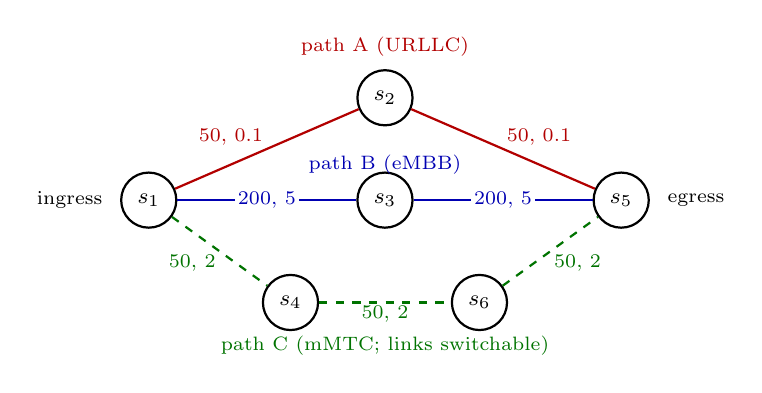
\begin{tikzpicture}[
  sw/.style={circle,draw,thick,minimum size=7mm,inner sep=0pt,font=\footnotesize},
  lk/.style={thick},
  lbl/.style={font=\scriptsize,fill=white,inner sep=1pt}]
\node[sw] (s1) at (0,0) {$s_1$};
\node[sw] (s2) at (3,1.3) {$s_2$};
\node[sw] (s3) at (3,0) {$s_3$};
\node[sw] (s4) at (1.8,-1.3) {$s_4$};
\node[sw] (s6) at (4.2,-1.3) {$s_6$};
\node[sw] (s5) at (6,0) {$s_5$};
\draw[lk,red!70!black] (s1) -- node[lbl,above left]{50, 0.1} (s2);
\draw[lk,red!70!black] (s2) -- node[lbl,above right]{50, 0.1} (s5);
\draw[lk,blue!70!black] (s1) -- node[lbl]{200, 5} (s3);
\draw[lk,blue!70!black] (s3) -- node[lbl]{200, 5} (s5);
\draw[lk,green!45!black,dashed] (s1) -- node[lbl,below left]{50, 2} (s4);
\draw[lk,green!45!black,dashed] (s4) -- node[lbl,below]{50, 2} (s6);
\draw[lk,green!45!black,dashed] (s6) -- node[lbl,below right]{50, 2} (s5);
\node[font=\scriptsize,left=1mm of s1] {ingress};
\node[font=\scriptsize,right=1mm of s5] {egress};
\node[font=\scriptsize,red!70!black] at (3,1.95) {path A (URLLC)};
\node[font=\scriptsize,blue!70!black] at (3,0.45) {path B (eMBB)};
\node[font=\scriptsize,green!45!black] at (3,-1.85) {path C (mMTC; links switchable)};
\end{tikzpicture}
\caption{Evaluation topology. Labels give link capacity (Mbit/s) and propagation
delay (ms). Path C's links can be powered off by the controller.}
\label{fig:topology}
\end{figure}

\begin{table}[t]
\caption{Scenarios (60 one-second slots each)}
\label{tab:scenarios}
\centering
\footnotesize
\begin{tabular}{@{}lp{6.2cm}@{}}
\toprule
s1 & No disturbance (control case). \\
s2 & 120\,Mbit/s of unmanaged traffic on path B, slots 20--40. \\
s3 & 35\,Mbit/s of unmanaged traffic on path A, slots 20--40. \\
s4 & eMBB demand $+50\,\%$ (15--35); telemetry frozen (20--30); background counters missing (40--45). \\
s5 & Model mismatch: true URLLC packets 1500\,B and mMTC 500\,B where the model assumes 64\,B and 100\,B; 20\,\% latency noise. \\
s6 & The s2 surge, plus a one-slot actuation delay throughout and a controller outage (45--50). \\
\bottomrule
\end{tabular}
\end{table}

% =====================================================================
\section{System Model}
\label{sec:system}

Time is slotted, $t \in \{0,1,\dots\}$, with slot length $\Delta t = 1$\,s.
Table~\ref{tab:notation} summarizes the notation.

\emph{State and demand.} The state $s_t$ is a set of 45 named, timestamped
measurements: per link the utilization and the background load (traffic outside the
managed slices); per slice the p99 latency, jitter, loss, throughput, queue occupancy
and active users; per switch the flow-table occupancy; and an energy proxy. Each
measurement carries the time it was taken, so stale values can be detected; missing
values stay missing. The exogenous input $d_t$ contains each slice's offered load
and number of active devices.

\emph{Action.} An action $a_t$ assigns to each slice $i \in \{\text{URLLC},
\text{eMBB}, \text{mMTC}\}$ a path $p_i$ from its allowed set, a rate budget $b_i$
within configured bounds (e.g.\ $b_{\mathrm{eMBB}} \in [1,150]$\,Mbit/s) and an
admission limit $n_i$, and sets an on/off state for each link of path C. The bounded
set of such actions is $\Acal$. All rates in the system, including budgets,
capacities and measurements, are Ethernet frame rates, which is what switch counters
and meters count.

\emph{Network.} The true transition $s_{t+1} = T(s_t, a_t, d_t, \varepsilon_t)$ is
unknown to the controller. In our experiments it is realized by one of two
evaluation environments, neither of which the controller models:
\begin{itemize}
\item a \emph{simulator} that computes per-slot ground truth from its own parameters
(true packet sizes, latency noise, overload with a 50\,ms buffer, scheduled
background, telemetry faults, actuation delays); and
\item an \emph{emulated network} on Mininet \cite{lantz2010mininet} with Open vSwitch
\cite{pfaff2015ovs}, programmed with OpenFlow~1.3 rules and meters
\cite{openflow13spec}, with shaped links, iperf3 traffic, 100 ping probes per slot
for latency, and switch counters for throughput and background load. It runs in real
time on one machine (Ubuntu 24.04 under WSL2, Mininet 2.3.0, Open vSwitch 3.3.9),
and its values are measurements, not ground truth.
\end{itemize}

\begin{table}[t]
\caption{Notation}
\label{tab:notation}
\centering
\footnotesize
\begin{tabular}{@{}lp{6.1cm}@{}}
\toprule
$s_t, d_t$ & measured state and demand at slot $t$ \\
$a_t \in \Acal$ & applied action; $\Acal$ the bounded action set \\
$p_i, b_i, n_i$ & path, rate budget, admission limit of slice $i$ \\
$T$ & true (unknown) transition: simulator or emulated network \\
$\That$ & nominal model used by the shield \\
$\dbar$ & demand forecast, $1.2\,d_t$ \\
$\pi_0$ & fallback policy \\
$\Ccal_t, \Ccal^\star_t$ & candidate set and its certified subset \\
$c(s,a)$ & hard-constraint vector, satisfied when $\le 0$ \\
$\varphi \in \Phi$ & STL intents; $\rho_\varphi$ local robustness \\
$H, \rhomin$ & rollout horizon (10 slots), robustness margin (0.05) \\
$V$ & shield: $V(s_t,d_t,a)\in\{0,1\}$ \\
\bottomrule
\end{tabular}
\end{table}

% =====================================================================
\section{Mathematical Formulation}
\label{sec:formulation}

This section states what the prototype computes. Bracketed equation numbers, e.g.\
[Eq.~17], refer to the course formulation \cite{vgcp_formulation}; where the
prototype interprets or replaces part of it, we say so. The formulation is
expressed in terms of a nominal model $\That$, which is \emph{not} the true
transition $T$: every quantity below with a hat is a prediction.

\subsection{Intents and robustness}
An intent is an STL formula over predicates $p(s,a)$. The prototype supports
single-signal predicates $x \le c$ and $x \ge c$ with value
\begin{equation}
p(s,a) = \frac{c - x(s,a)}{\sigma_x} \quad\text{or}\quad \frac{x(s,a) - c}{\sigma_x},
\label{eq:pred}
\end{equation}
where $\sigma_x$ is a declared scale for the signal's family (1\,ms for latency).
With $\sigma_x = 1$ this is [Eq.~6]; the scale makes robustness unitless, so one
margin $\rhomin$ can apply to intents with different units. Robustness follows the
standard quantitative semantics \cite{donze2010robust} [Eqs.~8--11]:
$\rho^{p}(\mathbf{s},\mathbf{a},t) = p(s_t,a_t)$,
$\rho^{\neg\varphi} = -\rho^{\varphi}$,
$\rho^{\varphi_1\wedge\varphi_2} = \min(\rho^{\varphi_1},\rho^{\varphi_2})$ and
\begin{equation}
\rho^{\varphi_1 \stlU_{[a,b]} \varphi_2}(t) =
\max_{\tau\in[t+a,t+b]} \min\Bigl(\rho^{\varphi_2}(\tau), \min_{u\in[t,\tau]} \rho^{\varphi_1}(u)\Bigr),
\end{equation}
with $\stlG_{[a,b]}\varphi = \neg(\top \stlU_{[a,b]} \neg\varphi)$ and time in
slots. The configured intents are
\begin{equation}
\varphi_i = \stlG_{[1,10]}\bigl(\text{latency}^{\mathrm{p99}}_i \le L_i\bigr),\quad
L = (1, 40, 20)\,\text{ms}.
\label{eq:intents}
\end{equation}
A missing sample makes the robustness unknown, which the shield treats as failure.

\subsection{Hard constraints}
The constraint vector $c(s,a)$ [Eq.~16] is satisfied when every component is
$\le 0$. For each link $\ell$ with capacity $C_\ell$,
\begin{equation}
c^{\mathrm{cap}}_\ell(s,a) = (1+\epsilon)\!\!\sum_{i:\,\ell \in p_i}\! b_i
 + B_\ell(s) - f_{\max} C_\ell ,
\label{eq:cap}
\end{equation}
where $B_\ell(s)$ is the measured background load, $f_{\max} = 0.9$ is the
reservation limit, and $\epsilon = 0.01$ accounts for a measured property of the
switch meters (Section~\ref{sec:meter}). Including $B_\ell$ is our reading of the
formulation's ``physical link capacities'': without it, traffic outside the managed
slices is invisible to the shield. The remaining components bound flow-table
occupancy (current occupancy plus two rules per slice routed through a switch, at
most 1000), enforce minimum budgets, and require each route to be an allowed,
loop-free ingress-to-egress path over powered-on links (0 if valid, 1 otherwise).

\subsection{Nominal model and projected rollout}
The formulation's learned world model $W_\psi$ [Eq.~22] is replaced by an analytic
model $\That$. With admitted fraction $f_i = \min(1, n_i/\text{devices}_i)$, the
predicted slice load is $x_i = \min\bigl(f_i\,\dbar_i,\,(1+\epsilon) b_i\bigr)$, the
link utilization is $u_\ell = (\sum_{i:\,\ell\in p_i} x_i + B_\ell)/C_\ell$, and the
predicted p99 latency of slice $i$ is
\begin{equation}
\hat{L}_i = k \sum_{\ell \in p_i} \Bigl( \delta_\ell + \delta_{\mathrm{proc}}
 + \ln(100)\, \frac{S_\ell}{1-u_\ell} \Bigr),
\label{eq:latency}
\end{equation}
where $\delta_\ell$ is the propagation delay, $\delta_{\mathrm{proc}} = 0.05$\,ms,
$S_\ell$ is the serialization time of the largest frame on $\ell$, and
$\ln(100)\,S/(1-u)$ is the 99th percentile of the M/M/1 sojourn time
\cite{kleinrock1975queueing}. Summing per-hop percentiles is a heuristic, not a
bound, and $k = 1.5$ is a safety factor that was set, not fitted. The model is valid
only while every $u_\ell \le 0.95$; outside that range its prediction is flagged.

Demand is forecast as a constant upper bound $\dbar_{t+k} = 1.2\, d_t$, and
background load is carried forward unchanged. Following [Eqs.~12--13], a candidate
$a$ is rolled forward for $H = 10$ steps:
\begin{equation}
\begin{aligned}
&\shat_t = s_t,\qquad \ahat_t = a,\\
&\shat_{t+k+1} = \That(\shat_{t+k}, \ahat_{t+k}, \dbar_{t+k}),\;\; k=0,\dots,H-1,\\
&\ahat_{t+k} = \pi_0(\shat_{t+k}),\;\; k\ge 1.
\end{aligned}
\label{eq:rollout}
\end{equation}

\subsection{Certification}
The local robustness of $a$ for intent $\varphi$ is its robustness on the projected
trajectory, $\rho_\varphi(s_t,a) = \rho^{\varphi}(\shat_{t:t+H}, \ahat_{t:t+H}, t)$
[Eq.~14]. The shield certifies $a$, $V(s_t,d_t,a) = 1$, if and only if
\begin{equation}
\begin{aligned}
& a \in \Acal \;\text{ and every input in } s_t, d_t \text{ is present,}\\
& \quad\text{finite, in range and fresh},\\
& c(s_t,a) \le 0 \;\text{ and }\; c(\shat_{t+k},\ahat_{t+k}) \le 0,\;\; k=1,\dots,H,\\
& \That \text{ in range and } \pi_0(\shat_{t+k}) \in \Acal \text{ at every step},\\
& \rho_\varphi(s_t,a) \ge \rhomin = 0.05 \quad \forall \varphi \in \Phi .
\end{aligned}
\label{eq:certify}
\end{equation}
Compared with the formulation's intent-feasible set $\Acal_\Phi(s)$ [Eq.~17], the
extra conditions in (\ref{eq:certify}) can only remove actions. Certification
therefore implies membership in $\Acal_\Phi(s_t)$ \emph{as computed with $\That$,
$\dbar$ and $\pi_0$}, which is the formulation's soundness property [Assumption~2]
relative to the model. It implies nothing about $T$.

Two interpretations are worth stating. First, (\ref{eq:intents}) uses
$\stlG_{[1,10]}$ rather than $\stlG_{[0,10]}$. Because [Eq.~14] starts at the
measured state, a violation already present at $t$ would make every action
uncertifiable, including the fallback that would correct it; excusing only the
measured slot still checks the candidate, whose effect first appears at $k=1$.
Second, the uncertainty trigger $u_\psi > \eta$ [Def.~2] needs a learned model; its
nearest Stage-1 analogue is the condition that $\That$ stays in its valid range.

\subsection{Fallback policy}
The fallback $\pi_0$ is separate from certification: it is what the applier installs
when nothing is certified, and it is not certified by construction. It starts from a
base action (URLLC on A, eMBB on B at 100\,Mbit/s, mMTC on C). If eMBB's path has
room, i.e.\
\begin{equation}
\min_{\ell\in p_{\mathrm{eMBB}}}\Bigl(f_{\max}C_\ell - B_\ell
 - (1+\epsilon)\!\!\sum_{i\neq \mathrm{eMBB}:\,\ell\in p_i}\!\! b_i\Bigr)
\ge (1+\epsilon)\, b_{\mathrm{eMBB}},
\label{eq:fbroom}
\end{equation}
it returns the base action; otherwise it moves eMBB to the allowed path with the most
room and shrinks its budget to fit. If any background load is unknown, it returns the
base action. The formulation assumes $\pi_0(s) \in \Acal_\Phi(s)$ for every
reachable $s$ [Assumption~3]. We do not establish this; whenever $\pi_0$ is applied,
we record whether the shield would have certified it.

\subsection{Selection and closed loop}
Let $\Ccal_t = (a^{(1)},\dots,a^{(K)})$ be the candidates in the generator's order
and $\Ccal^\star_t = \{a\in\Ccal_t : V(s_t,d_t,a)=1\}$ the certified ones. Selection
operates only on $\Ccal^\star_t$, so it cannot weaken certification. The
\emph{first-certified} rule takes the first element of $\Ccal^\star_t$. The
\emph{utility} rule implements [Eq.~42] with the deterministic $\That$, so the
expectation reduces to one rollout:
\begin{equation}
\sigma(s_t) = \arg\max_{a\in\Ccal^\star_t} \sum_{k=0}^{H}
\gamma^k\, U(\shat_{t+k}, \ahat_{t+k}),\quad \gamma = 0.9,
\label{eq:select}
\end{equation}
\begin{equation}
U(s,a) = \alpha_1 \frac{\sum_i \mathrm{thr}_i(s)}{100} - \alpha_2 \frac{E(s)}{10}
 + \alpha_3 \min_{p} p(s,a) - \alpha_4 \frac{\sum_i b_i}{100},
\label{eq:utility}
\end{equation}
with $(\alpha_1,\alpha_2,\alpha_3,\alpha_4) = (1, 0.1, 1, 0.5)$, $E$ the energy
proxy, and the minimum over all intent predicates [Eq.~27]. The weights are
illustrative and were not tuned. The applied action and the closed loop are
\begin{equation}
\begin{gathered}
a_t = \begin{cases} \text{selected } a\in\Ccal^\star_t, & \Ccal^\star_t \neq \emptyset,\\
\pi_0(s_t), & \text{otherwise}, \end{cases}\\
s_{t+1} = T(s_t, a_t, d_t, \varepsilon_t).
\end{gathered}
\label{eq:closed}
\end{equation}
The certificate concerns $\That$; the outcome in (\ref{eq:closed}) is produced by
$T$. The experiments measure the gap between the two.

% =====================================================================
\section{Methodology: The Shielded Control Loop}
\label{sec:method}

Each slot runs the same ten steps (Fig.~\ref{fig:loop}, Algorithm~\ref{alg:loop}):
(1)~observe telemetry; (2)~generate candidates; (3)~predict each candidate's
consequences with $\That$ and $\pi_0$; (4)~evaluate the hard constraints and the
STL intents on the prediction; (5)~compute robustness; (6)~certify the candidates
that pass; (7)~select one certified candidate; (8)~apply it through the certified
path, or the fallback if none passed; (9)~observe the resulting state in the next
slot; (10)~repeat. Keeping these steps separate is what lets the evaluation
attribute a violation to the generator, the model or the fallback.

\begin{figure}[t]
\centering
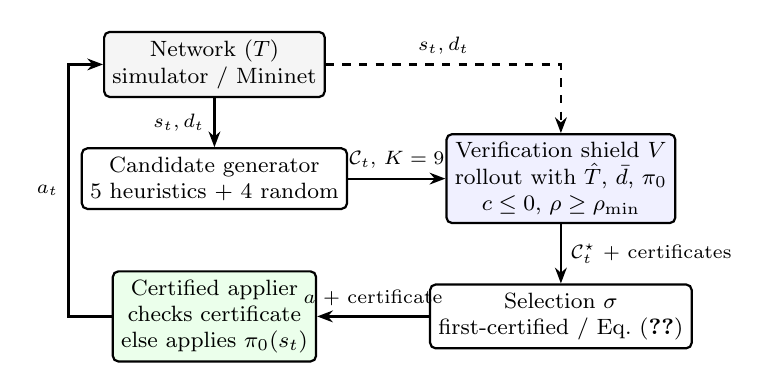
\begin{tikzpicture}[
  box/.style={draw,rounded corners=2pt,thick,align=center,font=\footnotesize,minimum height=7mm,inner sep=3pt},
  arr/.style={-{Stealth[length=2mm]},thick},
  note/.style={font=\scriptsize,align=center}]
\node[box,fill=gray!8] (net) at (0,0) {Network ($T$)\\ simulator / Mininet};
\node[box] (gen) at (0,-1.45) {Candidate generator\\ 5 heuristics + 4 random};
\node[box,fill=blue!6] (sh) at (4.4,-1.45) {Verification shield $V$\\ rollout with $\That$, $\dbar$, $\pi_0$\\ $c\le0$, $\rho\ge\rhomin$};
\node[box] (sel) at (4.4,-3.2) {Selection $\sigma$\\ first-certified / Eq.~(\ref{eq:select})};
\node[box,fill=green!8] (app) at (0,-3.2) {Certified applier\\ checks certificate\\ else applies $\pi_0(s_t)$};
\draw[arr] (net) -- node[note,left]{$s_t,d_t$} (gen);
\draw[arr] (gen) -- node[note,above]{$\Ccal_t$, $K=9$} (sh);
\draw[arr] (sh) -- node[note,right]{$\Ccal^\star_t$ + certificates} (sel);
\draw[arr] (sel) -- node[note,above]{$a$ + certificate} (app);
\draw[arr] (app.west) -- ++(-0.55,0) |- node[note,pos=0.25,left]{$a_t$} (net.west);
\draw[arr,dashed] (net.east) -| node[note,pos=0.25,above]{$s_t, d_t$} (sh.north);
\end{tikzpicture}
\caption{One control slot. Only the applier can change the network on the shielded
path, and it accepts an action only with a certificate issued for exactly that action
and observation.}
\label{fig:loop}
\end{figure}

\subsection{Candidate generation (stand-in for the generative policy)}
The formulation's generative policy $G_\theta$ [Eq.~21] is not implemented. A
heuristic generator proposes nine candidates per slot in a fixed order of
preference: \emph{greedy-embb} (eMBB budget at its maximum, 150\,Mbit/s),
\emph{demand-matched} (each budget $1.25\times$ the measured offered load),
\emph{capacity-fitted} (eMBB on the path with the most reservable room, budget
shrunk to fit), \emph{least-loaded-embb}, \emph{shortest-delay} (all slices on path
A), and four seeded random actions drawn uniformly from $\Acal$. The greedy
candidate comes first on purpose: it represents an aggressive generator, and the
random ones stand in for hallucinated proposals. Every candidate lies in $\Acal$, so
rejections come from predicted consequences, not from malformed actions. Missing
measurements are never read as zero: unknown demand keeps the fallback's budget, and a
link with unknown background is treated as full.

\subsection{Verification and certificates}
Algorithm~\ref{alg:shield} implements (\ref{eq:rollout})--(\ref{eq:certify}). Its
result is a certificate that lists every check with status pass, fail or unknown,
the robustness per intent, the constraint values, and fingerprints of the action,
state and demand it was issued for. An exception inside the shield yields an
unknown check, never acceptance.

\begin{algorithm}[t]
\caption{Verification shield $V(s_t, d_t, a)$}
\label{alg:shield}
\footnotesize
\begin{algorithmic}[1]
\State check $a\in\Acal$; check every input in $s_t,d_t$ is present, finite, in range and at most 2\,s old
\If{a check failed} \Return reject; mark remaining checks \emph{unknown} \EndIf
\State evaluate $c(s_t,a)$
\State $\dbar \gets 1.2\, d_t$; $\shat_t\gets s_t$; $\ahat_t\gets a$
\For{$k = 0,\dots,H-1$}
  \State $\shat_{t+k+1} \gets \That(\shat_{t+k},\ahat_{t+k},\dbar)$; record whether in range
  \State $\ahat_{t+k+1} \gets \pi_0(\shat_{t+k+1})$; check $\ahat_{t+k+1}\in\Acal$
\EndFor
\State evaluate $c(\shat_{t+k},\ahat_{t+k})$ for $k=1,\dots,H$
\If{$\That$ out of range or fallback invalid} \Return reject; intents \emph{unknown} \EndIf
\For{each $\varphi\in\Phi$} compute $\rho_\varphi$ on $(\shat,\ahat)_{t:t+H}$ \EndFor
\State \Return certificate: accept iff all checks pass and $\rho_\varphi\ge\rhomin\ \forall\varphi$; bind $a$, $s_t$, $d_t$, time
\end{algorithmic}
\end{algorithm}

\subsection{Selection and enforced application}
The applier is the only code path from a shielded controller to the network. It
refuses an action unless the certificate accepted exactly that action, was issued
for the same state and demand (by fingerprint), and is no older than a configured
limit. The one exception is the fallback: when nothing is certified, the applier
computes $\pi_0(s_t)$ itself, so no caller can pass another action off as the
fallback. The controller also asks the shield whether $\pi_0(s_t)$ would be
certified and records the answer; an \emph{uncertified fallback} is a slot in which
Assumption~3 failed.

\begin{algorithm}[t]
\caption{One slot of the shielded controller}
\label{alg:loop}
\footnotesize
\begin{algorithmic}[1]
\State observe $(s_t, d_t)$ \Comment{step 1}
\State $\Ccal_t \gets$ generator$(s_t,d_t)$ \Comment{step 2}
\State $\Ccal^\star_t \gets \{(a,\kappa) : \kappa \gets V(s_t,d_t,a),\ \kappa \text{ accepts}\}$ \Comment{steps 3--6}
\If{$\Ccal^\star_t\neq\emptyset$}
  \State $(a,\kappa) \gets$ first of $\Ccal^\star_t$, or $\sigma(s_t)$ of (\ref{eq:select}) \Comment{step 7}
  \State applier.apply\_certified$(a,\kappa,s_t,d_t)$ \Comment{step 8; refuses on mismatch}
\Else
  \State record $V(s_t,d_t,\pi_0(s_t))$; applier.apply\_fallback$(s_t)$ \Comment{step 8}
\EndIf
\State network advances one slot; outcome measured at $t+1$ \Comment{steps 9--10}
\end{algorithmic}
\end{algorithm}

\subsection{Model calibration}
To test whether the model's error is a scale error, a calibration tool computes, for
every recorded slot and slice, the ratio $r$ of recorded latency to the prediction of
(\ref{eq:latency}) with $k=1$, using that slot's own action, load and background. The
proposed factor is the 0.99-quantile of $r$ on training runs; its coverage, the
fraction of points with $k\hat{L}\ge L$, is then measured on runs it was not fitted
on. The adoption rule was fixed before fitting: a new factor replaces 1.5 only if it
reaches 99\,\% coverage on held-out seeds of the emulated network. A fit on the
simulator is reported but not adopted, since it would tune the shield to its own
evaluator.

\subsection{Implementation}
The prototype is about 6000 lines of Python 3.12, configured in YAML. Its 514 unit
tests include a check of the robustness computation against a direct implementation
of the recursive definitions [Eqs.~8--11], and a check of the shield against a
literal implementation of [Eq.~17] on a grid of 648 actions. Eleven further tests
run on the emulated network as root (meter policing, background accounting, reroute
timing, probe latency, counter freshness, frame-rate accounting, resource cleanup).
A dashboard runs the same loop slot by slot (Fig.~\ref{fig:dashboard}).

% =====================================================================
\section{Baseline Algorithms}
\label{sec:baselines}

All controllers receive the same nine candidates in the same order and act on the
same telemetry; they differ only in what they do with the candidates. This isolates
the effect of verification from the quality of the proposals.

\begin{itemize}
\item \textbf{shielded}: the proposed loop with first-certified selection.
\item \textbf{shielded-utility}: the proposed loop with utility selection
(\ref{eq:select}); comparing the two isolates the selection rule.
\item \textbf{unshielded}: applies greedy-embb, the generator's first choice, without
verification. Against \emph{shielded} it tests H1.
\item \textbf{unshielded-fitted}: applies the capacity-fitted candidate without
verification. It is a strong conventional heuristic and tests whether the shield
adds anything beyond a good hand-written rule.
\item \textbf{fallback-only}: always applies $\pi_0(s_t)$; it tests whether
candidates add anything beyond the fallback.
\end{itemize}

The unshielded baselines also run the shield in \emph{shadow mode}, without effect on
their action, to count applied actions the shield would have rejected. For H3, the
shielded and baseline controllers are repeated with a static fallback that always
restores the base action.

% =====================================================================
\section{Experimental Setup}
\label{sec:setup}

\emph{Simulation.} Every scenario in Table~\ref{tab:scenarios} was run with every
controller for seeds 1--5 (main campaign) and seeds 6--10 (held-out). The calibration
ablation repeats the held-out runs with the simulator-fitted factor $k = 1.109$ for
the controllers that use the shield, and the fallback ablation repeats seeds 1--5
with the static fallback. All simulation runs were made with the same code version
as the emulated s2 run below.

\emph{Emulated network.} Mininet campaigns covered s1--s3, the scenarios the
emulation supports without changes, with all five controllers in real time. We
report s2 for seeds 1--5 with the final implementation, and use an earlier s1--s3
campaign (seeds 1--5, before the meter correction) only for calibration and for the
latency issue in Section~\ref{sec:results}. Each campaign ran only after the eleven
root-only tests had passed twice in a row.

\emph{Metrics.} Outcomes are taken from the slot after each decision:
\emph{violation slots}, in which a link was overloaded (offered load above capacity)
or a slice's p99 latency exceeded its bound; \emph{reservation-limit slots}, with a
link above $0.9$ of capacity; \emph{fallback slots} and \emph{uncertified
fallbacks}; \emph{shadow rejections}; the \emph{candidate rejection rate};
\emph{reserved bandwidth} (sum of applied budgets); delivered eMBB throughput; and
verification time per slot. On the emulated network, overload cannot be observed
because shaped links never carry more than their capacity, and latency is the 99th
percentile of 100 probes. Values are mean $\pm$ standard deviation over seeds.

% Results and performance analysis.
% Sources (repository paths):
%   simulation, seeds 1-5 ............ experiments/reports/2026-11-09-sim-main/
%   simulation, held-out seeds 6-10 .. experiments/reports/2026-11-09-sim-heldout/
%   calibration ablation (k = 1.109) . experiments/reports/2026-11-09-sim-heldout-k1.109/
%   static-fallback ablation ......... experiments/reports/2026-11-09-sim-static/
%   simulator calibration ............ experiments/reports/2026-11-09-sim-main/calibration.md
%   Mininet s2 after meter fix ....... experiments/reports/2026-10-26-mininet-s2-meter-fix/
%   Mininet s1-s3 + calibration ...... experiments/reports/2026-10-26-mininet-s1-s3-5seeds/
%   meter and idle-latency tests ..... experiments/reports/2026-10-26-meter-sweep/
% All simulation runs: commit 296d117 (code identical to c831a00, used for the Mininet s2 run).

% =====================================================================
\section{Results}
\label{sec:results}

\subsection{H1: prevention (simulation)}

Table~\ref{tab:sim} gives the main campaign. Only s2 and s6 separate the
controllers: s1, s3 and s4 produced no violations for any controller, and s5
produced violations in every slot for every controller. The held-out seeds 6--10
reproduced every pattern in the table (s2: 0.8 against 16.4 violation slots; s6:
1.8 against 16.4).

\begin{table*}[t]
\caption{Simulation, seeds 1--5: mean $\pm$ std per 60-slot run. ``Viol.'' = violation slots; ``Fb'' = fallback slots (of which uncertified); ``Shadow'' = applied actions the shield would have rejected; ``Res.'' = mean reserved bandwidth (Mbit/s).}
\label{tab:sim}
\centering
\footnotesize
\setlength{\tabcolsep}{3.5pt}
\begin{tabular}{@{}l|ccc|ccc|cc|cc|cc@{}}
\toprule
& \multicolumn{3}{c|}{shielded} & \multicolumn{3}{c|}{shielded-utility} & \multicolumn{2}{c|}{unshielded} & \multicolumn{2}{c|}{unshielded-fitted} & \multicolumn{2}{c}{fallback-only}\\
Scen. & Viol. & Fb (unc.) & Res. & Viol. & Fb (unc.) & Res. & Viol. & Shadow & Viol. & Shadow & Viol. & Fb (unc.)\\
\midrule
s1 & 0 & 0 (0) & 155 & 0 & 0 (0) & 105 & 0 & 0 & 0 & 0 & 0 & 60 (0)\\
s2 & $0.8\pm0.4$ & 0 (0) & 124 & $0.8\pm0.4$ & 0 (0) & 91 & $16.4\pm1.1$ & 20 & $0.8\pm0.4$ & 0 & $0.8\pm0.4$ & 60 (0)\\
s3 & 0 & 20 (20) & 140 & 0 & 20 (20) & 107 & 0 & 20 & 0 & 20 & 0 & 60 (20)\\
s4 & 0 & 13 (13) & 145 & 0 & 13 (13) & 116 & 0 & 13 & 0 & 13 & 0 & 60 (13)\\
s5 & 60 & 0 (0) & 155 & 60 & 0 (0) & 105 & 60 & 0 & 60 & 0 & 60 & 60 (0)\\
s6 & $1.6\pm0.5$ & 0 (0) & 124 & $1.6\pm0.5$ & 0 (0) & 91 & $16.4\pm1.1$ & 20 & $1.6\pm0.5$ & 0 & $1.6\pm0.5$ & 60 (0)\\
\bottomrule
\end{tabular}
\end{table*}

\emph{What the shield prevents.} In s2 the unshielded controller applied the greedy
candidate (150\,Mbit/s for eMBB on path B) throughout the surge. Path B was
overloaded in 11.2 slots per run on average, eMBB latency exceeded its 40\,ms bound
in 16.4 slots, and recovery after the surge took 19 slots. In every one of the 20
surge slots the shield, running in shadow mode, would have rejected that action.
The shielded controller rejected the greedy candidate and applied a certified
capacity-fitted one; its only violation slot is the first slot of the surge, which
had been decided before the surge was observable (Fig.~\ref{fig:timeseries}). The
same pattern holds in s6, with one additional violation slot per run caused by the
one-slot actuation delay.

\emph{What it does not do.} The unverified capacity-fitted heuristic and the
fallback-only controller achieved exactly the same violation counts as the shielded
controllers in every scenario. In this setting, the shield's contribution is that
it made an aggressive, unchecked generator as safe as a carefully designed
heuristic, without having to trust the generator; it did not improve on the
heuristic. The price, relative to the unshielded controller, was eMBB throughput
during the surge: 72.8 against 79.8\,Mbit/s on average over the run.

\begin{figure}[t]
\centering
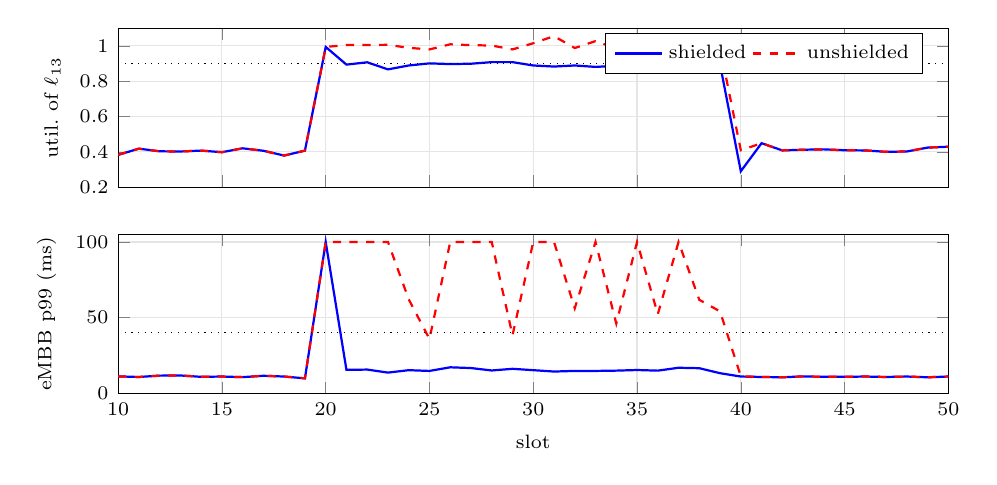
\begin{tikzpicture}
\begin{groupplot}[group style={group size=1 by 2, vertical sep=6mm, x descriptions at=edge bottom},
  width=\columnwidth, height=3.6cm, xmin=10, xmax=50, grid=major, grid style={gray!20},
  tick label style={font=\scriptsize}, label style={font=\scriptsize}, legend style={font=\scriptsize}]
\nextgroupplot[ylabel={util.\ of $\ell_{13}$}, ymin=0.2, ymax=1.1, legend pos=north east, legend columns=2]
\addplot[blue,thick] coordinates {(10,0.383) (11,0.418) (12,0.403) (13,0.402) (14,0.407) (15,0.398) (16,0.420) (17,0.406) (18,0.379) (19,0.407) (20,0.994) (21,0.894) (22,0.907) (23,0.867) (24,0.889) (25,0.901) (26,0.897) (27,0.899) (28,0.908) (29,0.908) (30,0.889) (31,0.883) (32,0.889) (33,0.881) (34,0.887) (35,0.876) (36,0.905) (37,0.895) (38,0.894) (39,0.895) (40,0.290) (41,0.449) (42,0.408) (43,0.412) (44,0.414) (45,0.409) (46,0.408) (47,0.400) (48,0.402) (49,0.424) (50,0.429)};
\addplot[red,thick,dashed] coordinates {(10,0.383) (11,0.418) (12,0.403) (13,0.402) (14,0.407) (15,0.398) (16,0.420) (17,0.406) (18,0.379) (19,0.407) (20,0.994) (21,1.005) (22,1.005) (23,1.006) (24,0.989) (25,0.980) (26,1.009) (27,1.004) (28,1.002) (29,0.980) (30,1.015) (31,1.055) (32,0.988) (33,1.027) (34,0.985) (35,0.996) (36,0.988) (37,1.018) (38,0.988) (39,0.989) (40,0.409) (41,0.449) (42,0.408) (43,0.412) (44,0.414) (45,0.409) (46,0.408) (47,0.400) (48,0.402) (49,0.424) (50,0.429)};
\addplot[black,thin,dotted,domain=10:50] {0.9};
\legend{shielded, unshielded}
\nextgroupplot[ylabel={eMBB p99 (ms)}, xlabel={slot}, ymin=0, ymax=105]
\addplot[blue,thick] coordinates {(10,11.2) (11,10.8) (12,11.7) (13,11.8) (14,10.9) (15,11.1) (16,10.7) (17,11.6) (18,11.1) (19,9.9) (20,100.0) (21,15.5) (22,15.7) (23,13.7) (24,15.3) (25,14.8) (26,17.2) (27,16.7) (28,15.1) (29,16.2) (30,15.3) (31,14.4) (32,14.8) (33,14.8) (34,15.0) (35,15.4) (36,15.0) (37,16.9) (38,16.6) (39,13.3) (40,11.1) (41,10.8) (42,10.6) (43,11.2) (44,10.9) (45,10.9) (46,11.1) (47,10.8) (48,11.1) (49,10.6) (50,11.1)};
\addplot[red,thick,dashed] coordinates {(10,11.2) (11,10.8) (12,11.7) (13,11.8) (14,10.9) (15,11.1) (16,10.7) (17,11.6) (18,11.1) (19,9.9) (20,100.0) (21,100.0) (22,100.0) (23,100.0) (24,62.1) (25,35.9) (26,100.0) (27,100.0) (28,100.0) (29,38.3) (30,100.0) (31,100.0) (32,56.2) (33,100.0) (34,46.1) (35,100.0) (36,52.3) (37,100.0) (38,61.8) (39,54.1) (40,11.3) (41,10.8) (42,10.6) (43,11.2) (44,10.9) (45,10.9) (46,11.1) (47,10.8) (48,11.1) (49,10.6) (50,11.1)};
\addplot[black,thin,dotted,domain=10:50] {40};
\end{groupplot}
\end{tikzpicture}
\caption{Scenario s2, seed 1 (simulation ground truth of each slot's outcome). The
surge occupies slots 20--40. Top: utilization of link $\ell_{13}$ on path B, with the
0.9 reservation limit. Bottom: eMBB p99 latency with its 40\,ms bound; values above
100\,ms (overloaded slots, up to 122\,ms) are clipped. Both controllers suffer the
surge's first slot, which was decided before it was observed.}
\label{fig:timeseries}
\end{figure}

\subsection{H3: fallback dependence}

Fig.~\ref{fig:fallback} compares the capacity-aware fallback with a static one that
always restores the base action (eMBB 100\,Mbit/s on path B). With the static
fallback, the shielded controller was exactly as bad as the unshielded one, 16.4
violation slots in both s2 and s6 (against 0.8 and 1.6 with the capacity-aware
fallback). The reason is visible in the certificates: during the surge no
candidate could be certified, because every rollout continues with $\pi_0$, and the
static $\pi_0$ itself breaks the capacity constraint at $k \ge 1$. The controller
therefore fell back in all 20 surge slots, to a fallback that was itself infeasible
(20 uncertified fallbacks). With the capacity-aware fallback, both the rollouts and
the fallback fit, and violations fell to 0.8. The generator, the model and the
verification logic were the same in both runs; only the fallback, and with it
Assumption~3, changed. The unshielded capacity-fitted heuristic, which does not use
$\pi_0$, was unaffected (0.8 and 1.6), and s1, s3 and s4 had the same violation and
fallback counts under both fallbacks.

\begin{figure}[t]
\centering
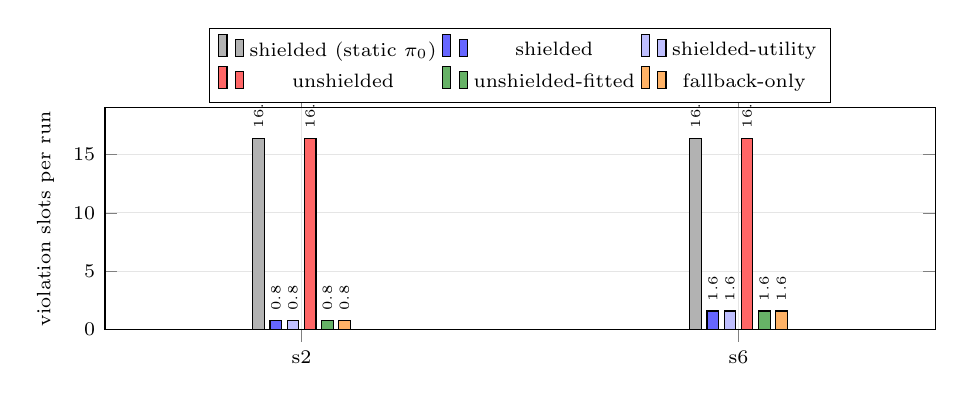
\begin{tikzpicture}
\begin{axis}[ybar, bar width=4.2pt, width=\columnwidth, height=4.4cm,
  ymin=0, ymax=19, ylabel={violation slots per run}, symbolic x coords={s2,s6},
  xtick=data, enlarge x limits=0.45, tick label style={font=\scriptsize},
  label style={font=\scriptsize}, legend style={font=\scriptsize, at={(0.5,1.02)}, anchor=south, legend columns=3},
  nodes near coords, every node near coord/.append style={font=\tiny, rotate=90, anchor=west},
  grid=major, grid style={gray!20}]
\addplot[fill=gray!60] coordinates {(s2,16.4) (s6,16.4)};
\addplot[fill=blue!60] coordinates {(s2,0.8) (s6,1.6)};
\addplot[fill=blue!25] coordinates {(s2,0.8) (s6,1.6)};
\addplot[fill=red!60] coordinates {(s2,16.4) (s6,16.4)};
\addplot[fill=green!50!black!60] coordinates {(s2,0.8) (s6,1.6)};
\addplot[fill=orange!60] coordinates {(s2,0.8) (s6,1.6)};
\legend{{shielded (static $\pi_0$)}, shielded, shielded-utility, unshielded, unshielded-fitted, fallback-only}
\end{axis}
\end{tikzpicture}
\caption{Violation slots in the two surge scenarios (simulation, seeds 1--5). The
first bar uses the static fallback; all others use the capacity-aware fallback.
In s1, s3 and s4 every controller had zero violation slots, and in s5 every
controller had 60.}
\label{fig:fallback}
\end{figure}

\subsection{Utility-based selection}

The two shielded controllers differ only in the selection rule. In every scenario
they had the same violations, fallbacks and delivered throughput (Table~\ref{tab:sim}),
but utility selection reserved 20--32\,\% less bandwidth: 155 against 105\,Mbit/s in
s1, 124 against 91 in s2, 145 against 116 in s4. Among the certified candidates it
chose demand-matched budgets where first-certified took the greedy one whenever
the greedy candidate was certifiable. In the simulator a budget above the offered
load does not change the outcome, so the only measured effect is the smaller
reservation. Since the utility weights are illustrative, this shows that the rule
works as specified, not that these weights are good.

\subsection{H2: model dependence and calibration}

\begin{table}[t]
\caption{Calibration of the latency safety factor $k$. Coverage: fraction of slot--slice points with $k\hat{L}\ge L_{\text{recorded}}$.}
\label{tab:calib}
\centering
\footnotesize
\setlength{\tabcolsep}{3pt}
\begin{tabular}{@{}llcc@{}}
\toprule
Data & Evaluated on & fitted $k$ & $k=1.5$\\
\midrule
\multicolumn{4}{@{}l}{\emph{Simulator}: fitted on seeds 1--5 of s1--s4, s6; $k=1.109$}\\
& held-out seeds 6--10, s1--s4, s6 & 98.3\,\% & 100\,\% \\
& s5 (model mismatch) & 39.6\,\% & 64.7\,\% \\
\midrule
\multicolumn{4}{@{}l}{\emph{Emulated network}: fitted on seeds 1--3 of s1--s3; $k=2.272$}\\
& held-out seeds 4--5, s1--s3 & 98.5\,\% & 95.3\,\% \\
\bottomrule
\end{tabular}
\end{table}

The configured factor $k=1.5$ was chosen, not fitted. On the simulator, the ratio of
recorded to predicted latency (with $k=1$) has a median of 1.00 and a 99th percentile
of 1.11 for every slice in the nominal scenarios, so $1.5$ is about 35\,\% more
pessimistic than necessary there. That pessimism is what causes the 20 uncertified
fallbacks in s3: the model predicts URLLC latency above 1\,ms on the loaded path A
while the simulated latency stays below it, so neither the candidates nor the
fallback can be certified. Re-running the held-out seeds with the fitted $k = 1.109$
removed all 20 fallbacks in s3, with no new violation and no other change in any
scenario.

The fit does not help in s5 (Table~\ref{tab:calib}). There the model assumes 64-byte
URLLC packets while the network sends 1500-byte packets, so the model's error is
structural, not a scale error, and no single factor fits it: coverage drops to
40\,\% with the fitted factor and is only 65\,\% with $k=1.5$. In s5 the shield
certified actions that violated the URLLC intent in all 60 slots, for every
controller.

On the emulated network, the factor fitted on seeds 1--3 was 2.27 and covered
98.5\,\% of the held-out slots, below the 99\,\% rule we had fixed in advance, so
$k=1.5$ was kept. We also did not adopt the simulator's $1.109$, since it would tune
the shield to its own evaluator. The emulated fit is driven by a heavy URLLC tail
(99th percentile of the ratio 3.7, maximum 17), which is related to the open
latency issue below.

\subsection{Emulated network}
\label{sec:meter}

\emph{Meter behaviour.} An earlier emulated campaign showed every controller
exceeding the 0.9 reservation limit in about 20 slots of s2, and metered eMBB slots
delivering 1.07 times their budget on average. A dedicated test isolated the cause
(Table~\ref{tab:meter}): an Open vSwitch meter that is left alone passes exactly its
budget, at any rate (1--70\,Mbit/s), frame size and burst size, but every
modification of the meter passes extra traffic in proportion to its burst size. The
controller modifies the eMBB meter almost every slot, because the certified budget
tracks the measured background. We reduced the meter burst from 0.1\,s to 0.01\,s
and kept the remaining 1\,\% in the model as $\epsilon$ in (\ref{eq:cap}), rather
than programming meters below their budget, which would have hidden the effect from
the shield.

\begin{table}[t]
\caption{Delivered/budget ratio of an Open vSwitch meter, offered 1.5$\times$ its budget, mean over six 1\,s slots (budgets 20 and 50\,Mbit/s gave the same values within 0.002).}
\label{tab:meter}
\centering
\footnotesize
\begin{tabular}{@{}lcc@{}}
\toprule
Meter burst & left unchanged & modified every slot\\
\midrule
0.01\,s & 0.998--0.999 & 1.005--1.006\\
0.1\,s (previous setting) & 1.000 & 1.066\\
1\,s & 1.000 & 1.495--1.497\\
\bottomrule
\end{tabular}
\end{table}

\emph{Scenario s2 after the correction.} Table~\ref{tab:mininet} reports s2 on the
emulated network with the final implementation. The pattern matches simulation:
the unshielded controller had the most violation slots and applied 20 actions per
run that the shield would have rejected, while the shielded controllers, the
capacity-fitted heuristic and the fallback stayed close to zero. Reservation-limit
slots fell from about 20 to about 4 per run after the meter correction; most of the
remainder fall in the first three slots of the surge, and the others exceed the
limit by small amounts consistent with measurement noise. With so few violations,
five seeds are not enough to rank the controllers other than the unshielded one.

\begin{table}[t]
\caption{Emulated network (Mininet/Open vSwitch), scenario s2, seeds 1--5, after the meter correction. Measured values, not ground truth; overload is not observable.}
\label{tab:mininet}
\centering
\footnotesize
\setlength{\tabcolsep}{2.5pt}
\begin{tabular}{@{}lccccc@{}}
\toprule
& shielded & sh.-utility & unshielded & uns.-fitted & fb-only\\
\midrule
Violation slots & $0.6\pm0.9$ & $0.8\pm1.3$ & $4.2\pm1.5$ & $1.2\pm1.8$ & $1.2\pm0.4$\\
Res.-limit slots & 4.0 & 4.6 & 20 & 3.8 & 3.4\\
Shadow rejections & 0 & 0 & 20 & 0 & 0\\
Rejection rate & 0.63 & 0.63 & -- & -- & --\\
Verify, p95 (ms) & 30 & 32 & 4 & 5 & 5\\
eMBB (Mbit/s) & 73.5 & 73.5 & 79.7 & 73.5 & 73.4\\
\bottomrule
\end{tabular}
\end{table}

\emph{Open issue: latency spikes.} In the s1--s3 campaign, which ran before the
meter correction, the URLLC p99 latency exceeded 1\,ms in 43 slots of s1 and 124
slots of s3 (summed over all 25 runs of each scenario), reaching 18.8\,ms on path A, whose propagation delay is 0.2\,ms. The
spikes affected every controller and clustered in individual runs (one shielded s1
run alone had 18 slots in which a slice exceeded its bound), so they are not attributable to the controllers.
On an idle path with the same 100 probes per slot, the per-slot p99 never exceeded
1\,ms (median 0.49\,ms), with or without the counter reads the backend performs each
slot. The spikes therefore require the campaign's traffic or host load, and their
cause is not yet known. For this reason we do not report controller comparisons for
s1 and s3 on the emulated network. Those scenarios have also not yet been repeated
with the meter correction.

\begin{figure*}[t]
\centering
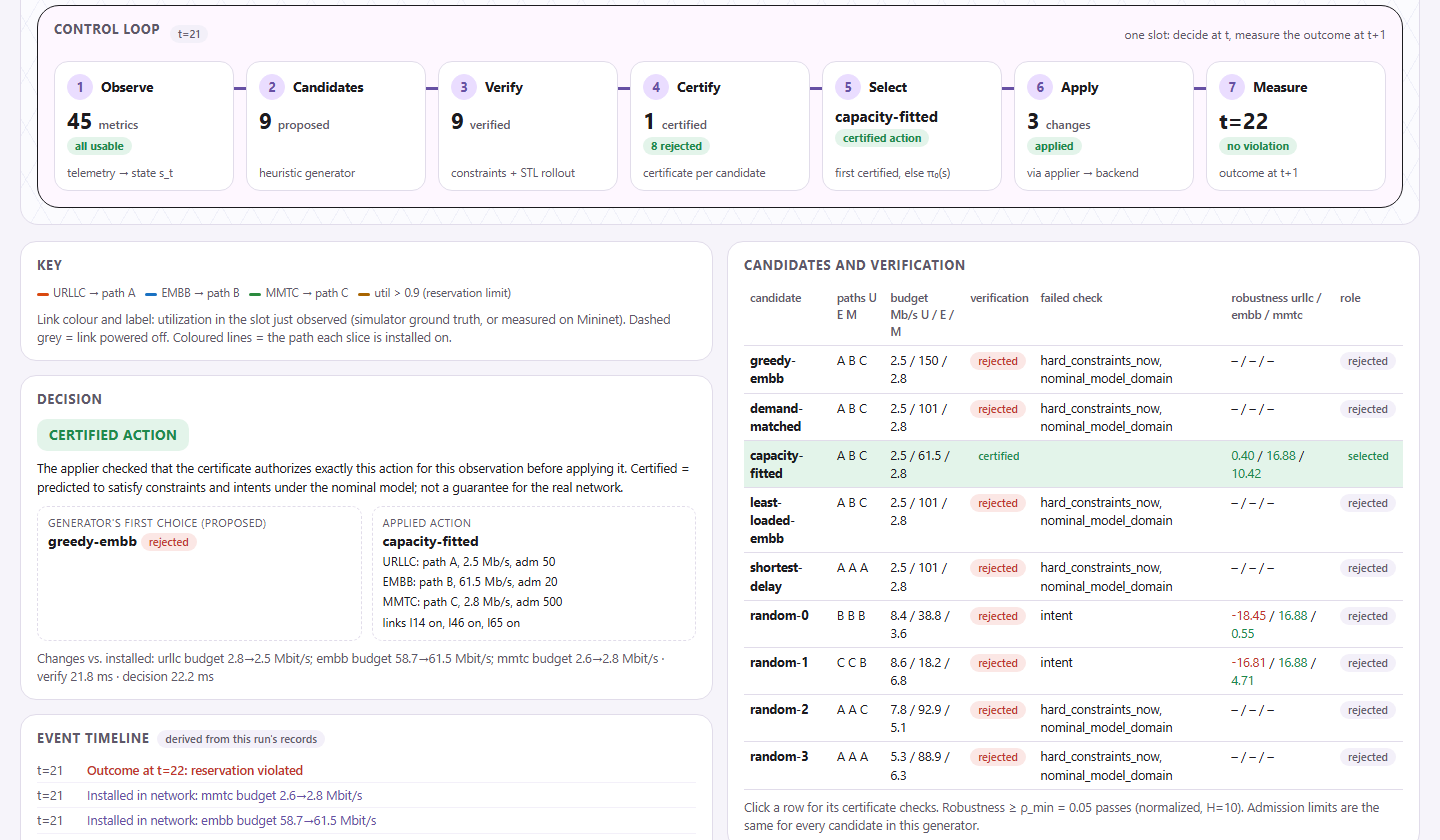
\includegraphics[width=0.92\textwidth]{figures/dashboard_slot.png}
\caption{The prototype's dashboard during one decision (scenario s2, slot 21,
simulation). Top: the seven stages of the slot. Left: the decision card, showing that
the generator's first choice (greedy-embb) was rejected and the certified
capacity-fitted candidate applied. Right: all nine candidates with the failed check
and the robustness per intent; two random candidates were rejected for the URLLC
intent with robustness $-18.5$ and $-16.8$, and the applied one had margins 0.40,
16.88 and 10.42 (all above $\rhomin = 0.05$). Verification of the nine candidates
took 21.8\,ms.}
\label{fig:dashboard}
\end{figure*}

% =====================================================================
\section{Performance Analysis}
\label{sec:analysis}

Table~\ref{tab:hyp} summarizes how the evidence bears on each hypothesis; the rest of
this section analyzes cost, filtering and the sources of the observed behaviour.

\begin{table}[t]
\caption{Hypotheses and evidence}
\label{tab:hyp}
\centering
\footnotesize
\setlength{\tabcolsep}{3pt}
\begin{tabular}{@{}p{0.9cm}p{4.5cm}p{2.3cm}@{}}
\toprule
& Evidence & Verdict \\
\midrule
H1 & s2: 16.4 $\to$ 0.8 violation slots (sim), 4.2 $\to$ 0.6 (emulated); s6: 16.4 $\to$ 1.6; held-out seeds agree & Supported; no gain over the capacity-aware heuristic \\
H2 & s5: certified actions violated URLLC in 60/60 slots; fitted $k$ covers 40\,\% of s5 & Supported \\
H3 & only $\pi_0$ changed: static gives 16.4 (s2, s6) with 20 uncertified fallbacks; capacity-aware gives 0.8 (s2), 1.6 (s6) & Supported \\
\bottomrule
\end{tabular}
\end{table}

\emph{Cost.} Verifying nine candidates, each with a ten-step rollout and three
intents, took 22--33\,ms at the 95th percentile per slot in simulation and about
30\,ms on the emulated network, against 3--5\,ms for the controllers without
verification. Utility selection adds one more rollout per certified candidate
(28--34\,ms). Both are small relative to a one-second slot, but the cost grows
linearly with the number of candidates and the horizon, so a generator that
proposes hundreds of candidates, or a stochastic model that needs many rollouts per
candidate, would change this picture.

\emph{Filtering.} The shield rejected 50\,\% of candidates in s1, 63\,\% in s2 and
s6, 61\,\% in s4 and 67\,\% in s3. In the surge slot shown in Fig.~\ref{fig:dashboard}, eight of nine candidates were
rejected: six for the capacity constraint together with the model's validity range,
and two random candidates for the URLLC intent. Measured against the formulation's Constraint 2, these are high rejection
rates, but they are rates for deliberately poor and random proposals, not for a
trained generator.

\emph{Where the safety came from.} Three observations together locate the source of
the improvement. With the static fallback the shield did not help; with the
capacity-aware fallback it did; and a capacity-aware heuristic achieved the same
result without the shield. The safety in the surge scenarios therefore comes from
having a decision that accounts for measured background load. What the shield adds
is that this property holds for whatever candidates are proposed, which the shadow
counts make concrete: 20 rejected actions per s2 run for the greedy generator, and
none for the heuristic.

\emph{Reaction lag.} Every controller pays for the first slot of a surge, because
the decision for that slot is made before the surge is measured. The shield
evaluates candidates against the current measurement and a constant forecast; it
cannot anticipate an event that the measurements do not show. Actuation delay (s6)
adds about one further slot, because the effect of a certified action falls outside
the window that was checked.

\emph{Conservatism versus safety.} In s3 and s4 the shield refused to certify
anything for 20 and 13 slots, although nothing would have been violated. In s3 this
is the pessimism of $k=1.5$ and disappears with a calibrated factor. In s4 it is the
intended behaviour on frozen or missing telemetry, at a cost of about 3\,\% eMBB
throughput relative to the unshielded controller. In s5 the opposite happened: the
model was optimistic, and the shield certified actions that were not safe. Both
failure directions are properties of the model, not of the verification logic.


% =====================================================================
\section{Limitations}
\label{sec:limits}

\begin{itemize}
\item \emph{No learned components.} The generator is heuristic and the model
analytic. The results say nothing about how often a learned generator's proposals
would be certified, or about the formulation's learned world model and its
uncertainty trigger.
\item \emph{Certification is relative to the model.} A certificate implies
feasibility only under $\That$, the forecast, $\pi_0$ and the configured
constraints; in s5 it was wrong in every slot.
\item \emph{The fallback is not guaranteed.} Recursive feasibility of $\pi_0$
(Assumption~3) is not established, and uncertified fallbacks occurred in s3 and s4.
\item \emph{Evaluation environments are not the real network.} The simulator shares
the shield's structural assumptions, and the emulated network runs on one machine.
Neither is evidence of safety in a production network.
\item \emph{Incomplete emulated evidence.} Only s2 has been run on the emulated
network with the final implementation; the s1--s3 campaign predates the meter
correction and shows latency spikes whose cause is unknown.
\item \emph{Scale and statistics.} One topology, one demand mix, five seeds per
campaign. Several cells have too few violations to rank controllers.
\item \emph{Illustrative parameters.} Thresholds, scales and utility weights were
chosen, not derived from requirements.
\end{itemize}

% =====================================================================
\section{Conclusion}

We asked whether predictive verification can keep candidate actions that violate
configured constraints or latency intents off the certified control path, and when
that protection fails. On the evaluated scenarios the answer has three parts.

\emph{H1 is supported where the model is adequate.} Given identical candidates,
routing them through the shield reduced violation slots under a background surge
from 16.4 to 0.8 per run in simulation (and from 4.2 to 0.6 on the emulated
network), because the shield rejected the greedy candidate in every surge slot, at
22--33\,ms per one-second slot. It did not improve on a capacity-aware heuristic,
which achieved the same outcomes without verification. What the certified path
contributes is that the outcome no longer depends on which candidate the generator
ranks first.

\emph{H2 is supported.} When the network differed structurally from the model, the
shield certified actions that violated the URLLC intent in all 60 slots, and a
recalibrated scale factor covered only 40\,\% of that scenario's points. Calibration
helped where the model's error was one of scale (it removed all 20 unnecessary
fallbacks of s3), but not where its structure was wrong.

\emph{H3 is supported.} Changing only the fallback, from capacity-aware to a fixed
one that did not fit the surge, raised the shielded controller's violation slots from
0.8 to 16.4 in s2 and from 1.6 to 16.4 in s6, the unshielded level: no rollout
continued by that fallback could be certified. The capacity-aware fallback is what made verification useful.

The prototype therefore demonstrates a certified path whose safety is a property of
the model and the fallback rather than of the generator. It does not demonstrate
safety on a real network, recursive feasibility of the fallback, or an advantage over
well-designed conventional control. The next steps follow from these results:
explain the remaining latency spikes on the emulated network and complete its
campaign, give the model uncertainty estimates that can trigger the fallback, for
example by conformal prediction \cite{angelopoulos2023conformal}, and only then
connect a learned generator to the same interface.

\bibliographystyle{IEEEtran}
\bibliography{references}

\end{document}
